\documentclass[11pt,letterpaper]{article}

% ============================================================================
% PACKAGES
% ============================================================================
\usepackage[utf8]{inputenc}
\usepackage[T1]{fontenc}
\usepackage{lmodern}
\usepackage[margin=1in]{geometry}
\usepackage{graphicx}
\usepackage{xcolor}
\usepackage{hyperref}
\usepackage{listings}
\usepackage{booktabs}
\usepackage{longtable}
\usepackage{array}
\usepackage{enumitem}
\usepackage{fancyhdr}
\usepackage{titlesec}
\usepackage{tocloft}
\usepackage{parskip}
\usepackage{float}
\usepackage{caption}
\usepackage{subcaption}
\usepackage{tikz}
\usetikzlibrary{shapes.geometric, arrows.meta, positioning, fit, backgrounds}

% ============================================================================
% COLOR DEFINITIONS
% ============================================================================
\definecolor{ghblue}{RGB}{36, 41, 47}
\definecolor{ghgreen}{RGB}{35, 134, 54}
\definecolor{ghorange}{RGB}{219, 109, 40}
\definecolor{ghpurple}{RGB}{130, 80, 223}
\definecolor{linkblue}{RGB}{0, 102, 204}
\definecolor{codebg}{RGB}{246, 248, 250}
\definecolor{codeframe}{RGB}{208, 215, 222}
\definecolor{commentgreen}{RGB}{106, 115, 125}
\definecolor{keywordblue}{RGB}{0, 92, 197}
\definecolor{stringbrown}{RGB}{163, 21, 21}

% ============================================================================
% HYPERREF CONFIGURATION
% ============================================================================
\hypersetup{
    colorlinks=true,
    linkcolor=ghblue,
    filecolor=ghpurple,
    urlcolor=linkblue,
    citecolor=ghgreen,
    pdftitle={Comprehensive Technical Implementation Guide: Automating GitHub Configuration Enforcement},
    pdfauthor={Technical Documentation},
    pdfsubject={GitHub Enterprise Configuration Management},
    pdfkeywords={GitHub, DevOps, Policy-as-Code, Configuration Management, Security}
}

% ============================================================================
% LISTINGS CONFIGURATION
% ============================================================================
\lstdefinestyle{yamlstyle}{
    backgroundcolor=\color{codebg},
    basicstyle=\ttfamily\small,
    breakatwhitespace=false,
    breaklines=true,
    captionpos=b,
    commentstyle=\color{commentgreen},
    frame=single,
    framerule=0.5pt,
    rulecolor=\color{codeframe},
    keepspaces=true,
    keywordstyle=\color{keywordblue}\bfseries,
    numbers=left,
    numbersep=8pt,
    numberstyle=\tiny\color{commentgreen},
    showspaces=false,
    showstringspaces=false,
    showtabs=false,
    stringstyle=\color{stringbrown},
    tabsize=2,
    xleftmargin=15pt,
    framexleftmargin=15pt
}

\lstdefinestyle{bashstyle}{
    backgroundcolor=\color{codebg},
    basicstyle=\ttfamily\small,
    breakatwhitespace=false,
    breaklines=true,
    captionpos=b,
    commentstyle=\color{commentgreen}\itshape,
    frame=single,
    framerule=0.5pt,
    rulecolor=\color{codeframe},
    keepspaces=true,
    keywordstyle=\color{keywordblue}\bfseries,
    morekeywords={gh, git, curl, jq, echo, if, then, fi, for, do, done, function},
    numbers=left,
    numbersep=8pt,
    numberstyle=\tiny\color{commentgreen},
    showspaces=false,
    showstringspaces=false,
    showtabs=false,
    stringstyle=\color{stringbrown},
    tabsize=2,
    xleftmargin=15pt,
    framexleftmargin=15pt,
    morecomment=[l]{\#}
}

\lstdefinestyle{jsonstyle}{
    backgroundcolor=\color{codebg},
    basicstyle=\ttfamily\small,
    breakatwhitespace=false,
    breaklines=true,
    captionpos=b,
    frame=single,
    framerule=0.5pt,
    rulecolor=\color{codeframe},
    keepspaces=true,
    keywordstyle=\color{keywordblue},
    numbers=left,
    numbersep=8pt,
    numberstyle=\tiny\color{commentgreen},
    showspaces=false,
    showstringspaces=false,
    showtabs=false,
    stringstyle=\color{stringbrown},
    tabsize=2,
    xleftmargin=15pt,
    framexleftmargin=15pt
}

\lstset{style=yamlstyle}

% ============================================================================
% HEADER/FOOTER CONFIGURATION
% ============================================================================
\pagestyle{fancy}
\fancyhf{}
\fancyhead[L]{\leftmark}
\fancyhead[R]{GitHub Configuration Enforcement}
\fancyfoot[C]{\thepage}
\renewcommand{\headrulewidth}{0.4pt}
\renewcommand{\footrulewidth}{0.4pt}

% ============================================================================
% SECTION FORMATTING
% ============================================================================
\titleformat{\section}
    {\normalfont\Large\bfseries\color{ghblue}}
    {\thesection}{1em}{}
\titleformat{\subsection}
    {\normalfont\large\bfseries\color{ghblue}}
    {\thesubsection}{1em}{}
\titleformat{\subsubsection}
    {\normalfont\normalsize\bfseries\color{ghblue}}
    {\thesubsubsection}{1em}{}

% ============================================================================
% CUSTOM COMMANDS
% ============================================================================
\newcommand{\ghurl}[2]{\href{#1}{\textcolor{linkblue}{#2}}}
\newcommand{\filepath}[1]{\texttt{\textcolor{ghpurple}{#1}}}
\newcommand{\apiendpoint}[1]{\texttt{\textcolor{ghorange}{#1}}}
\newcommand{\important}[1]{\textbf{\textcolor{ghgreen}{#1}}}
\newcommand{\warning}[1]{\textbf{\textcolor{ghorange}{Warning:}} #1}
\newcommand{\note}[1]{\textbf{\textcolor{ghblue}{Note:}} #1}

% ============================================================================
% DOCUMENT BEGIN
% ============================================================================
\begin{document}

% ============================================================================
% TITLE PAGE
% ============================================================================
\begin{titlepage}
    \centering
    \vspace*{2cm}
    
    {\Huge\bfseries\color{ghblue} Comprehensive Technical\\[0.3cm] Implementation Guide\par}
    \vspace{1cm}
    {\LARGE Automating Enforcement of\\[0.2cm] GitHub Configuration Files\par}
    
    \vspace{2cm}
    
    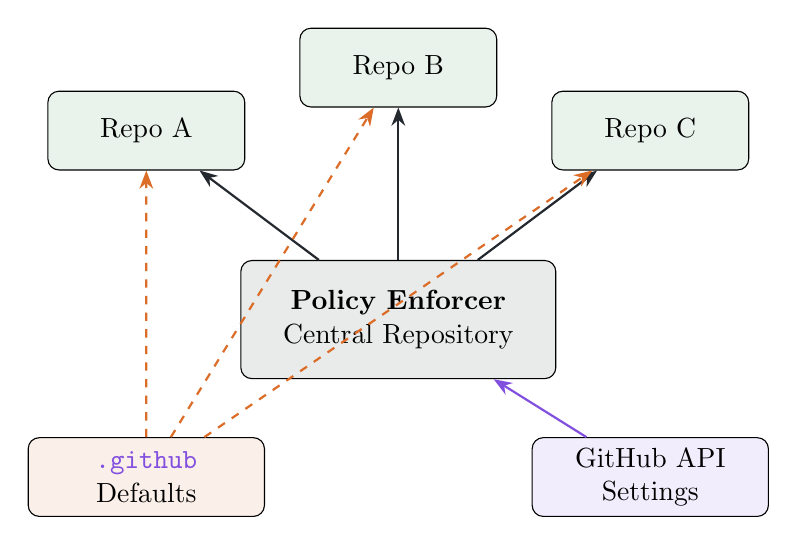
\begin{tikzpicture}[scale=0.8]
        % Central node
        \node[draw, rounded corners, fill=ghblue!10, minimum width=4cm, minimum height=1.5cm, align=center] (policy) at (0,0) {\textbf{Policy Enforcer}\\Central Repository};
        
        % Surrounding nodes
        \node[draw, rounded corners, fill=ghgreen!10, minimum width=2.5cm, minimum height=1cm, align=center] (repo1) at (-4,3) {Repo A};
        \node[draw, rounded corners, fill=ghgreen!10, minimum width=2.5cm, minimum height=1cm, align=center] (repo2) at (0,4) {Repo B};
        \node[draw, rounded corners, fill=ghgreen!10, minimum width=2.5cm, minimum height=1cm, align=center] (repo3) at (4,3) {Repo C};
        \node[draw, rounded corners, fill=ghorange!10, minimum width=3cm, minimum height=1cm, align=center] (dotgithub) at (-4,-2.5) {\filepath{.github}\\Defaults};
        \node[draw, rounded corners, fill=ghpurple!10, minimum width=3cm, minimum height=1cm, align=center] (api) at (4,-2.5) {GitHub API\\Settings};
        
        % Arrows
        \draw[-{Stealth}, thick, ghblue] (policy) -- (repo1);
        \draw[-{Stealth}, thick, ghblue] (policy) -- (repo2);
        \draw[-{Stealth}, thick, ghblue] (policy) -- (repo3);
        \draw[-{Stealth}, thick, ghorange, dashed] (dotgithub) -- (repo1);
        \draw[-{Stealth}, thick, ghorange, dashed] (dotgithub) -- (repo2);
        \draw[-{Stealth}, thick, ghorange, dashed] (dotgithub) -- (repo3);
        \draw[{Stealth}-, thick, ghpurple] (policy) -- (api);
    \end{tikzpicture}
    
    \vspace{2cm}
    
    {\large\itshape Policy-as-Code Implementation for\\Enterprise GitHub Organizations\par}
    
    \vfill
    
    {\large Version 1.0\par}
    {\large January 2026\par}
    
\end{titlepage}

% ============================================================================
% TABLE OF CONTENTS
% ============================================================================
\tableofcontents
\newpage

% ============================================================================
% SECTION 1: INTRODUCTION
% ============================================================================
\section{Introduction}
\label{sec:introduction}

This document provides a comprehensive technical implementation guide for automating the enforcement of GitHub configuration files across an enterprise organization. The approach treats configuration management as two distinct control surfaces: \textbf{file-based artifacts} (Markdown, YAML, and other files committed to repositories) and \textbf{setting-based controls} (repository and organization security settings managed via the GitHub API).

The implementation strategy encompasses three core pillars:

\begin{enumerate}[label=\textbf{\arabic*.}]
    \item \textbf{Centralized Defaults} --- Leveraging GitHub's native support for organization-level default community health files
    \item \textbf{Drift Detection} --- Automated auditing to identify repositories that deviate from organizational standards
    \item \textbf{Remediation via Pull Requests} --- Automated correction through PR-based synchronization with full audit trails
\end{enumerate}

These pillars are reinforced by \textbf{rulesets and status checks} that prevent repositories from drifting once brought into compliance.

\subsection{Scope of Configuration Files}

This guide addresses automation for the following 25 categories of GitHub configuration artifacts:

\begin{longtable}{@{}clp{8cm}@{}}
\toprule
\textbf{\#} & \textbf{Category} & \textbf{Configuration Items} \\
\midrule
\endhead
1--8 & Community Health & \filepath{CODE\_OF\_CONDUCT.md}, \filepath{CONTRIBUTING.md}, \filepath{SECURITY.md}, \filepath{SUPPORT.md}, \filepath{CITATION.cff}, \filepath{FUNDING.yml}, \filepath{CNAME}, Repository Description \\
\midrule
9--13 & Templates & Issue templates, PR templates, Issue forms, Discussion category forms, Template configuration \\
\midrule
14--18 & Workflows \& Ownership & Reusable workflows, Composite actions, Job summaries, \filepath{CODEOWNERS}, Starter workflow templates \\
\midrule
19--22 & Security & GHAS overview, Dependabot configuration, Secret scanning, Code scanning (CodeQL) \\
\midrule
23--25 & Releases & Latest release automation, Release notes generation, Release request forms \\
\midrule
26--28 & Profile READMEs & User profile README, Organization public profile, Organization member-only profile \\
\bottomrule
\end{longtable}

\subsection{Official Documentation References}

Throughout this guide, references to official GitHub documentation are provided. Key documentation hubs include:

\begin{itemize}[leftmargin=2cm]
    \item \ghurl{https://docs.github.com/en/communities/setting-up-your-project-for-healthy-contributions}{Community Health Files Documentation}
    \item \ghurl{https://docs.github.com/en/code-security}{Code Security Documentation}
    \item \ghurl{https://docs.github.com/en/actions}{GitHub Actions Documentation}
    \item \ghurl{https://docs.github.com/en/rest}{GitHub REST API Reference}
    \item \ghurl{https://docs.github.com/en/repositories/configuring-branches-and-merges-in-your-repository/managing-rulesets}{Repository Rulesets Documentation}
\end{itemize}

% ============================================================================
% SECTION 2: ARCHITECTURE OVERVIEW
% ============================================================================
\section{Architecture Overview}
\label{sec:architecture}

The enforcement architecture separates concerns into distinct layers, each with specific responsibilities and implementation patterns.

\subsection{Control Surface Classification}

\subsubsection{File-Based Artifacts}

File-based artifacts are configuration files that exist within repository file trees and are enforced through file synchronization. These include:

\begin{table}[H]
\centering
\caption{File-Based Configuration Artifacts}
\label{tab:file-artifacts}
\begin{tabular}{@{}lll@{}}
\toprule
\textbf{Category} & \textbf{File Path} & \textbf{Documentation} \\
\midrule
GitHub Pages & \filepath{CNAME} & \ghurl{https://docs.github.com/en/pages/configuring-a-custom-domain-for-your-github-pages-site/managing-a-custom-domain-for-your-github-pages-site}{Custom Domains} \\
\addlinespace
Code of Conduct & \filepath{CODE\_OF\_CONDUCT.md} & \ghurl{https://docs.github.com/en/communities/setting-up-your-project-for-healthy-contributions/adding-a-code-of-conduct-to-your-project}{Adding a Code of Conduct} \\
\addlinespace
Contributing Guide & \filepath{CONTRIBUTING.md} & \ghurl{https://docs.github.com/en/communities/setting-up-your-project-for-healthy-contributions/setting-guidelines-for-repository-contributors}{Contributor Guidelines} \\
\addlinespace
Security Policy & \filepath{SECURITY.md} & \ghurl{https://docs.github.com/en/code-security/getting-started/adding-a-security-policy-to-your-repository}{Security Policy} \\
\addlinespace
Support Resources & \filepath{SUPPORT.md} & \ghurl{https://docs.github.com/en/communities/setting-up-your-project-for-healthy-contributions/adding-support-resources-to-your-project}{Support Resources} \\
\addlinespace
Citation File & \filepath{CITATION.cff} & \ghurl{https://docs.github.com/en/repositories/managing-your-repositorys-settings-and-features/customizing-your-repository/about-citation-files}{Citation Files} \\
\addlinespace
Funding Config & \filepath{.github/FUNDING.yml} & \ghurl{https://docs.github.com/en/repositories/managing-your-repositorys-settings-and-features/customizing-your-repository/displaying-a-sponsor-button-in-your-repository}{Sponsor Button} \\
\bottomrule
\end{tabular}
\end{table}

\subsubsection{Template Files}

Issue and pull request templates require specific directory structures:

\begin{table}[H]
\centering
\caption{Template File Locations}
\label{tab:templates}
\begin{tabular}{@{}lp{7cm}@{}}
\toprule
\textbf{Template Type} & \textbf{Path(s)} \\
\midrule
Issue Templates & \filepath{.github/ISSUE\_TEMPLATE/*.md} or \filepath{.github/ISSUE\_TEMPLATE/*.yml} \\
\addlinespace
Issue Template Config & \filepath{.github/ISSUE\_TEMPLATE/config.yml} \\
\addlinespace
PR Templates & \filepath{.github/PULL\_REQUEST\_TEMPLATE.md} or \filepath{.github/PULL\_REQUEST\_TEMPLATE/*.md} \\
\addlinespace
Discussion Forms & \filepath{.github/DISCUSSION\_TEMPLATE/*.yml} \\
\bottomrule
\end{tabular}
\end{table}

\note{Template configuration supports YAML form schema for enhanced user experience. See \ghurl{https://docs.github.com/en/communities/using-templates-to-encourage-useful-issues-and-pull-requests/syntax-for-githubs-form-schema}{Form Schema Syntax}.}

\subsubsection{Setting-Based Controls}

Setting-based controls are repository or organization configurations managed via the GitHub API rather than committed files:

\begin{table}[H]
\centering
\caption{API-Managed Settings}
\label{tab:api-settings}
\begin{tabular}{@{}lll@{}}
\toprule
\textbf{Setting} & \textbf{API Endpoint} & \textbf{Documentation} \\
\midrule
Repository Description & \apiendpoint{PATCH /repos/\{owner\}/\{repo\}} & \ghurl{https://docs.github.com/en/rest/repos/repos}{Repos API} \\
\addlinespace
Dependabot Alerts & \apiendpoint{PUT /repos/.../vulnerability-alerts} & \ghurl{https://docs.github.com/en/code-security/dependabot/dependabot-alerts/configuring-dependabot-alerts}{Dependabot Alerts} \\
\addlinespace
Secret Scanning & \apiendpoint{PATCH /repos/.../security\_and\_analysis} & \ghurl{https://docs.github.com/en/code-security/secret-scanning}{Secret Scanning} \\
\addlinespace
Code Scanning & Default Setup or Workflow & \ghurl{https://docs.github.com/en/code-security/code-scanning/enabling-code-scanning/configuring-default-setup-for-code-scanning}{Code Scanning Setup} \\
\addlinespace
Security Configurations & \apiendpoint{/orgs/\{org\}/code-security/configurations} & \ghurl{https://docs.github.com/en/rest/code-security/configurations}{Configurations API} \\
\bottomrule
\end{tabular}
\end{table}

\subsection{Reference Repository Architecture}

The recommended architecture consists of four specialized repositories:

\begin{figure}[H]
\centering
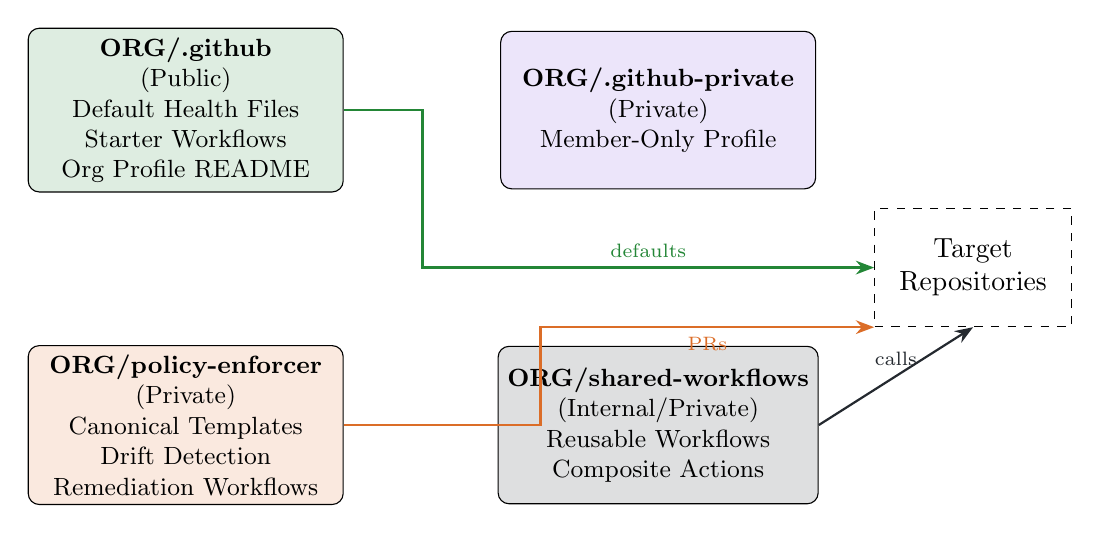
\begin{tikzpicture}[
    repo/.style={draw, rounded corners, minimum width=4cm, minimum height=2cm, align=center, font=\small},
    arrow/.style={-{Stealth}, thick}
]
    % Repositories
    \node[repo, fill=ghgreen!15] (dotgithub) at (0,0) {\textbf{ORG/.github}\\(Public)\\Default Health Files\\Starter Workflows\\Org Profile README};
    
    \node[repo, fill=ghpurple!15] (dotgithubprivate) at (6,0) {\textbf{ORG/.github-private}\\(Private)\\Member-Only Profile};
    
    \node[repo, fill=ghorange!15] (enforcer) at (0,-4) {\textbf{ORG/policy-enforcer}\\(Private)\\Canonical Templates\\Drift Detection\\Remediation Workflows};
    
    \node[repo, fill=ghblue!15] (shared) at (6,-4) {\textbf{ORG/shared-workflows}\\(Internal/Private)\\Reusable Workflows\\Composite Actions};
    
    % Target repos
    \node[draw, dashed, minimum width=2.5cm, minimum height=1.5cm, align=center] (targets) at (10,-2) {Target\\Repositories};
    
    % Arrows
    \draw[arrow, ghgreen] (dotgithub.east) -- ++(1,0) |- node[above, pos=0.75, font=\scriptsize] {defaults} (targets.west);
    \draw[arrow, ghorange] (enforcer.east) -- ++(2.5,0) |- node[below, pos=0.75, font=\scriptsize] {PRs} (targets.south west);
    \draw[arrow, ghblue] (shared.east) -- node[above, font=\scriptsize] {calls} (targets.south);
    
\end{tikzpicture}
\caption{Reference Repository Architecture}
\label{fig:repo-architecture}
\end{figure}

\subsubsection{ORG/.github Repository (Public)}

This repository serves as the central hub for organization-wide defaults:

\begin{lstlisting}[style=bashstyle, caption={.github Repository Structure}]
.github/
├── profile/
│   └── README.md              # Organization public profile
├── workflow-templates/
│   ├── ci-workflow.yml        # Starter workflow template
│   ├── ci-workflow.properties.json
│   ├── security-scan.yml
│   └── security-scan.properties.json
├── ISSUE_TEMPLATE/
│   ├── bug_report.yml
│   ├── feature_request.yml
│   └── config.yml
├── PULL_REQUEST_TEMPLATE.md
├── CODE_OF_CONDUCT.md
├── CONTRIBUTING.md
├── SECURITY.md
├── SUPPORT.md
└── FUNDING.yml
\end{lstlisting}

\important{Key Feature:} Files in this repository automatically serve as defaults for repositories that don't define their own versions. See \ghurl{https://docs.github.com/en/communities/setting-up-your-project-for-healthy-contributions/creating-a-default-community-health-file}{Creating Default Community Health Files}.

\subsubsection{ORG/.github-private Repository (Private)}

This private repository contains the member-only organization profile:

\begin{lstlisting}[style=bashstyle, caption={.github-private Repository Structure}]
.github-private/
└── profile/
    └── README.md    # Visible only to organization members
\end{lstlisting}

See \ghurl{https://docs.github.com/en/organizations/collaborating-with-groups-in-organizations/customizing-your-organizations-profile}{Customizing Organization Profile} for configuration details.

\subsubsection{ORG/policy-enforcer Repository (Private)}

The enforcement engine repository contains all automation logic:

\begin{lstlisting}[style=bashstyle, caption={policy-enforcer Repository Structure}]
policy-enforcer/
├── .github/
│   └── workflows/
│       ├── drift-detection.yml      # Scheduled audit workflow
│       ├── remediation.yml          # PR creation workflow
│       └── compliance-check.yml     # Reusable compliance check
├── templates/
│   ├── CODEOWNERS                   # Canonical CODEOWNERS template
│   ├── dependabot.yml               # Dependabot configuration
│   └── workflows/
│       └── codeql.yml               # CodeQL workflow template
├── config/
│   ├── inventory.yml                # Repository inventory
│   ├── exceptions.yml               # Policy exceptions
│   └── settings.yml                 # API settings to enforce
├── scripts/
│   ├── audit.sh                     # Drift detection script
│   ├── remediate.sh                 # PR creation script
│   └── api-settings.sh              # API settings enforcement
└── reports/
    └── .gitkeep                     # Generated reports directory
\end{lstlisting}

\subsubsection{ORG/shared-workflows Repository (Internal)}

Centralized reusable workflows accessible across the organization:

\begin{lstlisting}[style=bashstyle, caption={shared-workflows Repository Structure}]
shared-workflows/
└── .github/
    └── workflows/
        ├── reusable-ci.yml           # Reusable CI workflow
        ├── reusable-security.yml     # Reusable security scan
        ├── reusable-release.yml      # Reusable release workflow
        └── policy-compliance.yml     # Compliance status check
\end{lstlisting}

\warning{Repository visibility must be configured to allow workflow access. See \ghurl{https://docs.github.com/en/actions/creating-actions/sharing-actions-and-workflows-with-your-organization}{Sharing Workflows with Your Organization}.}

% ============================================================================
% SECTION 3: FILE-BASED ARTIFACT ENFORCEMENT
% ============================================================================
\section{File-Based Artifact Enforcement}
\label{sec:file-enforcement}

This section details the implementation of file-based artifact enforcement, covering each category of configuration files with specific templates and automation patterns.

\subsection{Community Health Files}

Community health files establish project governance and contributor expectations. GitHub recognizes these files from specific locations.

\subsubsection{CODE\_OF\_CONDUCT.md}

The code of conduct defines community standards and behavior expectations.

\begin{lstlisting}[caption={CODE\_OF\_CONDUCT.md Template}, language={}]
# Code of Conduct

## Our Pledge

We as members, contributors, and leaders pledge to make participation 
in our community a harassment-free experience for everyone.

## Our Standards

Examples of behavior that contributes to a positive environment:

- Using welcoming and inclusive language
- Being respectful of differing viewpoints and experiences
- Gracefully accepting constructive criticism
- Focusing on what is best for the community

## Enforcement

Instances of abusive, harassing, or otherwise unacceptable behavior 
may be reported to the community leaders responsible for enforcement 
at [INSERT CONTACT METHOD].

## Attribution

This Code of Conduct is adapted from the Contributor Covenant, 
version 2.1, available at 
https://www.contributor-covenant.org/version/2/1/code_of_conduct.html
\end{lstlisting}

\note{GitHub automatically detects Contributor Covenant and other standard codes of conduct. See \ghurl{https://docs.github.com/en/communities/setting-up-your-project-for-healthy-contributions/adding-a-code-of-conduct-to-your-project}{Adding a Code of Conduct}.}

\subsubsection{SECURITY.md}

The security policy provides vulnerability reporting instructions.

\begin{lstlisting}[caption={SECURITY.md Template}, language={}]
# Security Policy

## Supported Versions

| Version | Supported          |
| ------- | ------------------ |
| 5.1.x   | :white_check_mark: |
| 5.0.x   | :x:                |
| 4.0.x   | :white_check_mark: |
| < 4.0   | :x:                |

## Reporting a Vulnerability

To report a security vulnerability, please use the GitHub Security 
Advisory feature at:

https://github.com/ORG/REPO/security/advisories/new

**Do NOT report security vulnerabilities through public GitHub issues.**

### What to Include

- Type of issue (e.g., buffer overflow, SQL injection, XSS)
- Full paths of source file(s) related to the issue
- Location of affected source code (tag/branch/commit or URL)
- Step-by-step reproduction instructions
- Proof-of-concept or exploit code (if possible)
- Impact of the issue, including how it might be exploited

### Response Timeline

- Initial response: within 48 hours
- Status update: within 7 days
- Resolution target: within 90 days
\end{lstlisting}

See \ghurl{https://docs.github.com/en/code-security/getting-started/adding-a-security-policy-to-your-repository}{Adding a Security Policy} for integration with GitHub Security Advisories.

\subsubsection{CITATION.cff}

The Citation File Format enables proper academic citation.

\begin{lstlisting}[caption={CITATION.cff Template}, language={}]
cff-version: 1.2.0
title: "Project Name"
message: "If you use this software, please cite it as below."
type: software
authors:
  - family-names: "Lastname"
    given-names: "Firstname"
    orcid: "https://orcid.org/0000-0000-0000-0000"
    affiliation: "Organization Name"
repository-code: "https://github.com/ORG/REPO"
url: "https://project-website.org"
license: MIT
version: "1.0.0"
date-released: "2025-01-01"
keywords:
  - keyword1
  - keyword2
\end{lstlisting}

GitHub automatically parses \filepath{CITATION.cff} and provides citation export functionality. See \ghurl{https://docs.github.com/en/repositories/managing-your-repositorys-settings-and-features/customizing-your-repository/about-citation-files}{About Citation Files}.

\subsection{CODEOWNERS Configuration}

The \filepath{CODEOWNERS} file defines code ownership for automatic review assignment.

\begin{lstlisting}[caption={CODEOWNERS Template}, language={}]
# CODEOWNERS - Automatic review assignment
# Documentation: https://docs.github.com/articles/about-code-owners

# Default owners for everything in the repo
*       @org/platform-team

# Documentation
/docs/                          @org/docs-team
*.md                            @org/docs-team

# Source code by component
/src/api/                       @org/api-team
/src/frontend/                  @org/frontend-team
/src/backend/                   @org/backend-team

# Infrastructure and DevOps
/.github/                       @org/devops-team
/infrastructure/                @org/devops-team
Dockerfile                      @org/devops-team
docker-compose*.yml             @org/devops-team

# Security-sensitive files require security team review
/src/auth/                      @org/security-team @org/api-team
/src/crypto/                    @org/security-team
SECURITY.md                     @org/security-team

# Configuration files
*.yml                           @org/devops-team
*.yaml                          @org/devops-team
*.json                          @org/platform-team

# Build and dependencies
package.json                    @org/frontend-team @org/devops-team
requirements.txt                @org/backend-team @org/devops-team
go.mod                          @org/backend-team
go.sum                          @org/backend-team
\end{lstlisting}

\important{Location Requirements:} \filepath{CODEOWNERS} can be placed in the repository root, \filepath{docs/}, or \filepath{.github/} directory. GitHub checks these locations in order. See \ghurl{https://docs.github.com/en/repositories/managing-your-repositorys-settings-and-features/customizing-your-repository/about-code-owners}{About Code Owners}.

\subsection{Dependabot Configuration}

Dependabot automates dependency updates through \filepath{.github/dependabot.yml}.

\begin{lstlisting}[caption={dependabot.yml Template}]
# Dependabot configuration
# Docs: https://docs.github.com/en/code-security/dependabot

version: 2
registries:
  npm-private:
    type: npm-registry
    url: https://npm.pkg.github.com
    token: ${{ secrets.NPM_TOKEN }}
    replaces-base: false

updates:
  # JavaScript/TypeScript dependencies
  - package-ecosystem: "npm"
    directory: "/"
    schedule:
      interval: "weekly"
      day: "monday"
      time: "06:00"
      timezone: "America/New_York"
    open-pull-requests-limit: 10
    registries:
      - npm-private
    labels:
      - "dependencies"
      - "javascript"
    reviewers:
      - "org/frontend-team"
    assignees:
      - "octocat"
    commit-message:
      prefix: "deps"
      include: "scope"
    groups:
      development-dependencies:
        dependency-type: "development"
        update-types:
          - "minor"
          - "patch"
      production-dependencies:
        dependency-type: "production"
        update-types:
          - "patch"

  # Python dependencies
  - package-ecosystem: "pip"
    directory: "/"
    schedule:
      interval: "weekly"
    labels:
      - "dependencies"
      - "python"
    ignore:
      - dependency-name: "django"
        versions: ["4.x"]

  # GitHub Actions
  - package-ecosystem: "github-actions"
    directory: "/"
    schedule:
      interval: "weekly"
    labels:
      - "dependencies"
      - "github-actions"
    reviewers:
      - "org/devops-team"

  # Docker dependencies
  - package-ecosystem: "docker"
    directory: "/"
    schedule:
      interval: "weekly"
    labels:
      - "dependencies"
      - "docker"

  # Terraform modules
  - package-ecosystem: "terraform"
    directory: "/infrastructure"
    schedule:
      interval: "weekly"
\end{lstlisting}

See \ghurl{https://docs.github.com/en/code-security/dependabot/dependabot-version-updates/configuration-options-for-the-dependabot.yml-file}{Dependabot Configuration Options} for complete configuration reference.

\subsection{Issue and Pull Request Templates}

\subsubsection{Issue Form Templates (YAML)}

Modern issue templates use YAML form schema for structured input.

\begin{lstlisting}[caption={Bug Report Issue Form (.github/ISSUE\_TEMPLATE/bug\_report.yml)}]
name: Bug Report
description: File a bug report to help us improve
title: "[Bug]: "
labels: ["bug", "triage"]
assignees:
  - octocat
body:
  - type: markdown
    attributes:
      value: |
        Thanks for taking the time to fill out this bug report!
        
  - type: input
    id: version
    attributes:
      label: Version
      description: What version of our software are you running?
      placeholder: ex. 1.0.0
    validations:
      required: true
      
  - type: dropdown
    id: os
    attributes:
      label: Operating System
      description: What OS are you using?
      options:
        - Windows
        - macOS
        - Linux
        - Other
    validations:
      required: true
      
  - type: textarea
    id: what-happened
    attributes:
      label: What happened?
      description: Describe the bug and what you expected
      placeholder: Tell us what you see!
      value: |
        ## Current Behavior
        
        ## Expected Behavior
        
    validations:
      required: true
      
  - type: textarea
    id: reproduction
    attributes:
      label: Steps to Reproduce
      description: Steps to reproduce the behavior
      placeholder: |
        1. Go to '...'
        2. Click on '...'
        3. Scroll down to '...'
        4. See error
    validations:
      required: true
      
  - type: textarea
    id: logs
    attributes:
      label: Relevant log output
      description: Please copy and paste any relevant log output.
      render: shell
      
  - type: checkboxes
    id: terms
    attributes:
      label: Code of Conduct
      description: By submitting this issue, you agree to follow our CoC
      options:
        - label: I agree to follow this project's Code of Conduct
          required: true
\end{lstlisting}

See \ghurl{https://docs.github.com/en/communities/using-templates-to-encourage-useful-issues-and-pull-requests/syntax-for-githubs-form-schema}{GitHub Form Schema Syntax}.

\subsubsection{Issue Template Configuration}

The \filepath{config.yml} file controls template chooser behavior.

\begin{lstlisting}[caption={Issue Template Config (.github/ISSUE\_TEMPLATE/config.yml)}]
blank_issues_enabled: false
contact_links:
  - name: GitHub Community Support
    url: https://github.com/community/discussions
    about: Please ask and answer questions here.
  - name: Security Vulnerabilities
    url: https://github.com/ORG/REPO/security/advisories/new
    about: Please report security vulnerabilities here.
  - name: Stack Overflow
    url: https://stackoverflow.com/questions/tagged/project-name
    about: Ask questions on Stack Overflow.
\end{lstlisting}

See \ghurl{https://docs.github.com/en/communities/using-templates-to-encourage-useful-issues-and-pull-requests/configuring-issue-templates-for-your-repository}{Configuring Issue Templates}.

\subsubsection{Pull Request Template}

\begin{lstlisting}[caption={Pull Request Template (.github/PULL\_REQUEST\_TEMPLATE.md)}, language={}]
## Description

<!-- Describe your changes in detail -->

## Related Issue

<!-- Link to the issue this PR addresses -->
Fixes #

## Type of Change

<!-- Mark relevant options with [x] -->

- [ ] Bug fix (non-breaking change that fixes an issue)
- [ ] New feature (non-breaking change that adds functionality)
- [ ] Breaking change (fix or feature causing existing functionality change)
- [ ] Documentation update
- [ ] Refactoring (no functional changes)

## Checklist

- [ ] My code follows the project's style guidelines
- [ ] I have performed a self-review of my code
- [ ] I have commented my code, particularly in hard-to-understand areas
- [ ] I have made corresponding changes to the documentation
- [ ] My changes generate no new warnings
- [ ] I have added tests that prove my fix is effective or feature works
- [ ] New and existing unit tests pass locally with my changes
- [ ] Any dependent changes have been merged and published

## Screenshots (if applicable)

<!-- Add screenshots to help explain your changes -->

## Additional Notes

<!-- Any additional information for reviewers -->
\end{lstlisting}

See \ghurl{https://docs.github.com/en/communities/using-templates-to-encourage-useful-issues-and-pull-requests/creating-a-pull-request-template-for-your-repository}{Creating PR Templates}.

\subsection{Workflow Templates}

Starter workflow templates are stored in \filepath{.github/workflow-templates/}.

\subsubsection{Workflow Template File}

\begin{lstlisting}[caption={CI Workflow Template (workflow-templates/ci.yml)}]
name: CI Pipeline

on:
  push:
    branches: [$default-branch]
  pull_request:
    branches: [$default-branch]

permissions:
  contents: read
  pull-requests: write

jobs:
  build:
    runs-on: ubuntu-latest
    
    steps:
      - name: Checkout repository
        uses: actions/checkout@v4
        
      - name: Setup Node.js
        uses: actions/setup-node@v4
        with:
          node-version: '20'
          cache: 'npm'
          
      - name: Install dependencies
        run: npm ci
        
      - name: Run linting
        run: npm run lint
        
      - name: Run tests
        run: npm test
        
      - name: Build
        run: npm run build
\end{lstlisting}

\subsubsection{Workflow Template Metadata}

Each template requires a corresponding \filepath{.properties.json} file.

\begin{lstlisting}[style=jsonstyle, caption={Workflow Template Metadata (workflow-templates/ci.properties.json)}]
{
  "name": "Organization CI Pipeline",
  "description": "Standard CI workflow for organization projects",
  "iconName": "octicon workflow",
  "categories": [
    "JavaScript",
    "TypeScript",
    "Node"
  ],
  "filePatterns": [
    "package.json"
  ]
}
\end{lstlisting}

See \ghurl{https://docs.github.com/en/actions/using-workflows/creating-starter-workflows-for-your-organization}{Creating Starter Workflows for Your Organization}.

\subsection{Code Scanning Configuration}

\subsubsection{CodeQL Workflow (Advanced Setup)}

\begin{lstlisting}[caption={CodeQL Workflow (.github/workflows/codeql.yml)}]
name: "CodeQL Analysis"

on:
  push:
    branches: [main, develop]
  pull_request:
    branches: [main, develop]
  schedule:
    - cron: '30 1 * * 1'  # Weekly on Monday at 1:30 AM

permissions:
  security-events: write
  packages: read
  actions: read
  contents: read

jobs:
  analyze:
    name: Analyze (${{ matrix.language }})
    runs-on: ${{ matrix.os }}
    timeout-minutes: 360
    
    strategy:
      fail-fast: false
      matrix:
        include:
          - language: javascript-typescript
            os: ubuntu-latest
            build-mode: none
          - language: python
            os: ubuntu-latest
            build-mode: none
          - language: go
            os: ubuntu-latest
            build-mode: autobuild
            
    steps:
      - name: Checkout repository
        uses: actions/checkout@v4
        
      - name: Initialize CodeQL
        uses: github/codeql-action/init@v3
        with:
          languages: ${{ matrix.language }}
          build-mode: ${{ matrix.build-mode }}
          queries: +security-extended,security-and-quality
          
      - if: matrix.build-mode == 'manual'
        name: Manual Build
        shell: bash
        run: |
          echo 'Manual build commands here'
          
      - name: Perform CodeQL Analysis
        uses: github/codeql-action/analyze@v3
        with:
          category: "/language:${{ matrix.language }}"
          upload: true
\end{lstlisting}

\note{For simpler setups, consider using CodeQL default setup which requires no workflow file. See \ghurl{https://docs.github.com/en/code-security/code-scanning/enabling-code-scanning/configuring-default-setup-for-code-scanning}{Configuring Default Setup for Code Scanning}.}

% ============================================================================
% SECTION 4: SETTING-BASED ENFORCEMENT
% ============================================================================
\section{Setting-Based Enforcement via API}
\label{sec:api-enforcement}

This section covers enforcement of repository settings that are managed through the GitHub API rather than committed files.

\subsection{Repository Security Settings}

\subsubsection{Enable Security Features}

\begin{lstlisting}[style=bashstyle, caption={Enable Repository Security Features}]
#!/bin/bash
# Enable security features for a repository
# Docs: https://docs.github.com/en/rest/repos/repos

ORG="your-organization"
REPO="your-repository"

# Enable Dependabot alerts
gh api \
  --method PUT \
  -H "Accept: application/vnd.github+json" \
  "/repos/${ORG}/${REPO}/vulnerability-alerts"

# Enable Dependabot security updates
gh api \
  --method PUT \
  -H "Accept: application/vnd.github+json" \
  "/repos/${ORG}/${REPO}/automated-security-fixes"

# Enable secret scanning and push protection
gh api \
  --method PATCH \
  -H "Accept: application/vnd.github+json" \
  "/repos/${ORG}/${REPO}" \
  -f security_and_analysis='{"secret_scanning":{"status":"enabled"},"secret_scanning_push_protection":{"status":"enabled"}}'
\end{lstlisting}

See \ghurl{https://docs.github.com/en/code-security/secret-scanning/enabling-secret-scanning-features/enabling-secret-scanning-for-your-repository}{Enabling Secret Scanning}.

\subsubsection{Configure Code Security at Organization Scale}

GitHub provides code security configurations for applying consistent settings across multiple repositories.

\begin{lstlisting}[style=bashstyle, caption={Create Organization Security Configuration}]
#!/bin/bash
# Create a code security configuration
# Docs: https://docs.github.com/en/rest/code-security/configurations

ORG="your-organization"

# Create configuration
gh api \
  --method POST \
  -H "Accept: application/vnd.github+json" \
  "/orgs/${ORG}/code-security/configurations" \
  -f name="Standard Security Config" \
  -f description="Default security settings for all repositories" \
  -f advanced_security="enabled" \
  -f dependency_graph="enabled" \
  -f dependabot_alerts="enabled" \
  -f dependabot_security_updates="enabled" \
  -f secret_scanning="enabled" \
  -f secret_scanning_push_protection="enabled" \
  -f code_scanning_default_setup="enabled" \
  -f enforcement="enforced"

# Attach configuration to repositories
CONFIG_ID="12345"  # From previous response
gh api \
  --method POST \
  -H "Accept: application/vnd.github+json" \
  "/orgs/${ORG}/code-security/configurations/${CONFIG_ID}/attach" \
  -f scope="all"
\end{lstlisting}

See \ghurl{https://docs.github.com/en/code-security/securing-your-organization/enabling-security-features-in-your-organization/applying-a-custom-security-configuration}{Applying Security Configurations}.

\subsection{Repository Metadata Updates}

\begin{lstlisting}[style=bashstyle, caption={Update Repository Metadata}]
#!/bin/bash
# Update repository description, topics, and settings
# Docs: https://docs.github.com/en/rest/repos/repos

ORG="your-organization"
REPO="your-repository"

# Update description and homepage
gh api \
  --method PATCH \
  -H "Accept: application/vnd.github+json" \
  "/repos/${ORG}/${REPO}" \
  -f description="Official project description" \
  -f homepage="https://project.example.com" \
  -F has_issues=true \
  -F has_projects=true \
  -F has_wiki=false \
  -F allow_squash_merge=true \
  -F allow_merge_commit=false \
  -F allow_rebase_merge=true \
  -F delete_branch_on_merge=true

# Update topics
gh api \
  --method PUT \
  -H "Accept: application/vnd.github+json" \
  "/repos/${ORG}/${REPO}/topics" \
  -f names='["python","api","internal-tool"]'
\end{lstlisting}

\subsection{Enable CodeQL Default Setup}

\begin{lstlisting}[style=bashstyle, caption={Enable CodeQL Default Setup}]
#!/bin/bash
# Enable CodeQL default setup for a repository
# Docs: https://docs.github.com/en/code-security/code-scanning

ORG="your-organization"
REPO="your-repository"

gh api \
  --method PATCH \
  -H "Accept: application/vnd.github+json" \
  "/repos/${ORG}/${REPO}/code-scanning/default-setup" \
  -f state="configured" \
  -f query_suite="default" \
  -f languages='["javascript","python"]'
\end{lstlisting}

% ============================================================================
% SECTION 5: DRIFT DETECTION IMPLEMENTATION
% ============================================================================
\section{Drift Detection Implementation}
\label{sec:drift-detection}

Drift detection identifies repositories that have deviated from organizational standards. This section provides complete implementation details.

\subsection{Audit Workflow}

\begin{lstlisting}[caption={Drift Detection Workflow (.github/workflows/drift-detection.yml)}]
name: Policy Drift Detection

on:
  schedule:
    - cron: '0 6 * * 1'  # Weekly on Monday at 6 AM UTC
  workflow_dispatch:
    inputs:
      target_repo:
        description: 'Specific repository to audit (optional)'
        required: false
        type: string
      dry_run:
        description: 'Run in dry-run mode (no PRs)'
        required: false
        type: boolean
        default: true

permissions:
  contents: read
  issues: write
  pull-requests: write

env:
  POLICY_VERSION: "v1.2.0"

jobs:
  enumerate-repos:
    name: Enumerate Repositories
    runs-on: ubuntu-latest
    outputs:
      repos: ${{ steps.get-repos.outputs.repos }}
      
    steps:
      - name: Checkout policy-enforcer
        uses: actions/checkout@v4
        
      - name: Get repository list
        id: get-repos
        env:
          GH_TOKEN: ${{ secrets.ORG_ADMIN_TOKEN }}
        run: |
          if [ -n "${{ inputs.target_repo }}" ]; then
            echo "repos=[\"${{ inputs.target_repo }}\"]" >> $GITHUB_OUTPUT
          else
            # Get all non-archived, non-fork repositories
            repos=$(gh repo list ${{ github.repository_owner }} \
              --no-archived \
              --source \
              --json nameWithOwner \
              --limit 500 \
              -q '[.[].nameWithOwner]')
            echo "repos=${repos}" >> $GITHUB_OUTPUT
          fi

  audit:
    name: Audit Repository
    needs: enumerate-repos
    runs-on: ubuntu-latest
    strategy:
      fail-fast: false
      max-parallel: 5
      matrix:
        repo: ${{ fromJson(needs.enumerate-repos.outputs.repos) }}
        
    steps:
      - name: Checkout policy-enforcer
        uses: actions/checkout@v4
        
      - name: Checkout target repository
        uses: actions/checkout@v4
        with:
          repository: ${{ matrix.repo }}
          path: target-repo
          token: ${{ secrets.ORG_ADMIN_TOKEN }}
          
      - name: Run audit checks
        id: audit
        env:
          GH_TOKEN: ${{ secrets.ORG_ADMIN_TOKEN }}
          TARGET_REPO: ${{ matrix.repo }}
        run: |
          chmod +x scripts/audit.sh
          ./scripts/audit.sh target-repo > audit-report.json
          
      - name: Check for drift
        id: drift
        run: |
          drift=$(jq '.has_drift' audit-report.json)
          echo "has_drift=${drift}" >> $GITHUB_OUTPUT
          
      - name: Upload audit report
        uses: actions/upload-artifact@v4
        with:
          name: audit-${{ hashFiles('audit-report.json') }}
          path: audit-report.json
          retention-days: 30

  generate-report:
    name: Generate Summary Report
    needs: audit
    runs-on: ubuntu-latest
    if: always()
    
    steps:
      - name: Download all audit reports
        uses: actions/download-artifact@v4
        with:
          pattern: audit-*
          path: reports/
          
      - name: Generate summary
        run: |
          echo "# Policy Drift Detection Report" > summary.md
          echo "" >> summary.md
          echo "**Date:** $(date -u +"%Y-%m-%d %H:%M:%S UTC")" >> summary.md
          echo "**Policy Version:** ${{ env.POLICY_VERSION }}" >> summary.md
          echo "" >> summary.md
          
          # Aggregate results
          compliant=0
          drifted=0
          for report in reports/*/audit-report.json; do
            if [ -f "$report" ]; then
              if jq -e '.has_drift == true' "$report" > /dev/null; then
                ((drifted++))
              else
                ((compliant++))
              fi
            fi
          done
          
          echo "## Summary" >> summary.md
          echo "- Compliant: ${compliant}" >> summary.md
          echo "- Drifted: ${drifted}" >> summary.md
          
      - name: Create or update tracking issue
        env:
          GH_TOKEN: ${{ secrets.GITHUB_TOKEN }}
        run: |
          gh issue create \
            --title "Policy Drift Report - $(date +%Y-%m-%d)" \
            --body-file summary.md \
            --label "policy-drift,automated"
\end{lstlisting}

\subsection{Audit Script Implementation}

\begin{lstlisting}[style=bashstyle, caption={Audit Script (scripts/audit.sh)}]
#!/bin/bash
# Policy compliance audit script
# Usage: ./audit.sh <repo-path>

set -euo pipefail

REPO_PATH="${1:-.}"
REPORT_FILE="${2:-/dev/stdout}"

# Initialize report
declare -A checks
has_drift=false

# Check function
check_file() {
    local file="$1"
    local required="${2:-true}"
    local description="$3"
    
    if [ -f "${REPO_PATH}/${file}" ]; then
        checks["${file}"]="present"
    elif [ "${required}" = "true" ]; then
        checks["${file}"]="missing"
        has_drift=true
    else
        checks["${file}"]="optional-missing"
    fi
}

# Check for required files
check_file "CODE_OF_CONDUCT.md" "false" "Code of Conduct"
check_file "CONTRIBUTING.md" "false" "Contributing Guidelines"
check_file "SECURITY.md" "true" "Security Policy"
check_file "SUPPORT.md" "false" "Support Resources"
check_file ".github/CODEOWNERS" "true" "Code Owners"
check_file ".github/dependabot.yml" "true" "Dependabot Config"
check_file ".github/PULL_REQUEST_TEMPLATE.md" "true" "PR Template"

# Check for issue templates
if [ -d "${REPO_PATH}/.github/ISSUE_TEMPLATE" ]; then
    template_count=$(find "${REPO_PATH}/.github/ISSUE_TEMPLATE" \
        -name "*.yml" -o -name "*.md" 2>/dev/null | wc -l)
    if [ "$template_count" -gt 0 ]; then
        checks["issue_templates"]="present"
    else
        checks["issue_templates"]="empty"
        has_drift=true
    fi
else
    checks["issue_templates"]="missing"
    has_drift=true
fi

# Check CODEOWNERS validity
if [ -f "${REPO_PATH}/.github/CODEOWNERS" ]; then
    # Verify CODEOWNERS has valid team references
    invalid_refs=$(grep -E '^[^#].*@' "${REPO_PATH}/.github/CODEOWNERS" | \
        grep -v '@org/' || true)
    if [ -n "$invalid_refs" ]; then
        checks["codeowners_valid"]="invalid-teams"
        has_drift=true
    else
        checks["codeowners_valid"]="valid"
    fi
fi

# Check security settings via API
if [ -n "${GH_TOKEN:-}" ] && [ -n "${TARGET_REPO:-}" ]; then
    # Check Dependabot alerts
    dependabot_status=$(gh api "/repos/${TARGET_REPO}/vulnerability-alerts" \
        --silent 2>&1 && echo "enabled" || echo "disabled")
    checks["dependabot_alerts"]="${dependabot_status}"
    [ "${dependabot_status}" = "disabled" ] && has_drift=true
    
    # Check secret scanning
    secret_scan=$(gh api "/repos/${TARGET_REPO}" \
        --jq '.security_and_analysis.secret_scanning.status // "disabled"')
    checks["secret_scanning"]="${secret_scan}"
    [ "${secret_scan}" != "enabled" ] && has_drift=true
    
    # Check push protection
    push_protect=$(gh api "/repos/${TARGET_REPO}" \
        --jq '.security_and_analysis.secret_scanning_push_protection.status // "disabled"')
    checks["push_protection"]="${push_protect}"
    [ "${push_protect}" != "enabled" ] && has_drift=true
fi

# Generate JSON report
{
    echo "{"
    echo "  \"repository\": \"${TARGET_REPO:-unknown}\","
    echo "  \"audit_date\": \"$(date -u +"%Y-%m-%dT%H:%M:%SZ")\","
    echo "  \"has_drift\": ${has_drift},"
    echo "  \"checks\": {"
    
    first=true
    for key in "${!checks[@]}"; do
        [ "$first" = "true" ] && first=false || echo ","
        printf "    \"%s\": \"%s\"" "$key" "${checks[$key]}"
    done
    
    echo ""
    echo "  }"
    echo "}"
} > "${REPORT_FILE}"

# Exit with drift status
$has_drift && exit 1 || exit 0
\end{lstlisting}

% ============================================================================
% SECTION 6: REMEDIATION IMPLEMENTATION
% ============================================================================
\section{Remediation Implementation}
\label{sec:remediation}

The remediation system automatically creates pull requests to bring non-compliant repositories into conformance.

\subsection{Remediation Workflow}

\begin{lstlisting}[caption={Remediation Workflow (.github/workflows/remediation.yml)}]
name: Policy Remediation

on:
  workflow_dispatch:
    inputs:
      target_repo:
        description: 'Repository to remediate (owner/repo)'
        required: true
        type: string
      dry_run:
        description: 'Create draft PR instead of regular PR'
        required: false
        type: boolean
        default: true
      remediation_scope:
        description: 'Scope of remediation'
        required: true
        type: choice
        options:
          - all
          - files-only
          - settings-only
          - security-only

permissions:
  contents: write
  pull-requests: write

env:
  POLICY_BRANCH: "policy/sync-${{ github.run_id }}"

jobs:
  remediate:
    name: Remediate Repository
    runs-on: ubuntu-latest
    
    steps:
      - name: Checkout policy-enforcer
        uses: actions/checkout@v4
        path: enforcer
        
      - name: Checkout target repository
        uses: actions/checkout@v4
        with:
          repository: ${{ inputs.target_repo }}
          path: target
          token: ${{ secrets.ORG_ADMIN_TOKEN }}
          
      - name: Create remediation branch
        working-directory: target
        run: |
          git checkout -b ${{ env.POLICY_BRANCH }}
          
      - name: Sync CODEOWNERS
        if: inputs.remediation_scope == 'all' || inputs.remediation_scope == 'files-only'
        run: |
          mkdir -p target/.github
          
          # Check if repo has specific CODEOWNERS needs
          if [ -f "enforcer/config/codeowners-overrides.yml" ]; then
            repo_key=$(echo "${{ inputs.target_repo }}" | tr '/' '_')
            override=$(yq ".overrides.${repo_key} // empty" \
              enforcer/config/codeowners-overrides.yml)
            if [ -n "$override" ]; then
              echo "Using override CODEOWNERS for ${{ inputs.target_repo }}"
              cp "enforcer/templates/codeowners/${override}" target/.github/CODEOWNERS
            else
              cp enforcer/templates/CODEOWNERS target/.github/CODEOWNERS
            fi
          else
            cp enforcer/templates/CODEOWNERS target/.github/CODEOWNERS
          fi
          
      - name: Sync Dependabot configuration
        if: inputs.remediation_scope == 'all' || inputs.remediation_scope == 'files-only'
        run: |
          mkdir -p target/.github
          
          # Detect package ecosystems
          ecosystems=""
          [ -f "target/package.json" ] && ecosystems="${ecosystems}npm,"
          [ -f "target/requirements.txt" ] && ecosystems="${ecosystems}pip,"
          [ -f "target/go.mod" ] && ecosystems="${ecosystems}gomod,"
          [ -f "target/Gemfile" ] && ecosystems="${ecosystems}bundler,"
          [ -f "target/pom.xml" ] && ecosystems="${ecosystems}maven,"
          [ -f "target/Cargo.toml" ] && ecosystems="${ecosystems}cargo,"
          [ -d "target/.github/workflows" ] && ecosystems="${ecosystems}github-actions,"
          [ -f "target/Dockerfile" ] && ecosystems="${ecosystems}docker,"
          
          # Generate dependabot.yml based on detected ecosystems
          python3 enforcer/scripts/generate-dependabot.py \
            --ecosystems "${ecosystems}" \
            --output target/.github/dependabot.yml
            
      - name: Sync issue templates
        if: inputs.remediation_scope == 'all' || inputs.remediation_scope == 'files-only'
        run: |
          mkdir -p target/.github/ISSUE_TEMPLATE
          cp -r enforcer/templates/ISSUE_TEMPLATE/* target/.github/ISSUE_TEMPLATE/
          
      - name: Sync PR template
        if: inputs.remediation_scope == 'all' || inputs.remediation_scope == 'files-only'
        run: |
          cp enforcer/templates/PULL_REQUEST_TEMPLATE.md \
            target/.github/PULL_REQUEST_TEMPLATE.md
            
      - name: Sync security policy
        if: inputs.remediation_scope == 'all' || inputs.remediation_scope == 'files-only'
        run: |
          # Only sync if not already present (preserve custom policies)
          if [ ! -f "target/SECURITY.md" ]; then
            cp enforcer/templates/SECURITY.md target/SECURITY.md
          fi
          
      - name: Apply security settings
        if: inputs.remediation_scope == 'all' || inputs.remediation_scope == 'settings-only' || inputs.remediation_scope == 'security-only'
        env:
          GH_TOKEN: ${{ secrets.ORG_ADMIN_TOKEN }}
        run: |
          # Enable Dependabot alerts
          gh api --method PUT \
            "/repos/${{ inputs.target_repo }}/vulnerability-alerts" || true
            
          # Enable automated security fixes
          gh api --method PUT \
            "/repos/${{ inputs.target_repo }}/automated-security-fixes" || true
            
          # Enable secret scanning and push protection
          gh api --method PATCH \
            "/repos/${{ inputs.target_repo }}" \
            -f security_and_analysis='{"secret_scanning":{"status":"enabled"},"secret_scanning_push_protection":{"status":"enabled"}}' || true
            
          # Enable CodeQL default setup if applicable
          primary_lang=$(gh api "/repos/${{ inputs.target_repo }}/languages" \
            --jq 'to_entries | sort_by(.value) | reverse | .[0].key')
          
          case "$primary_lang" in
            JavaScript|TypeScript|Python|Go|Java|Ruby|C|C++|C#|Swift|Kotlin)
              gh api --method PATCH \
                "/repos/${{ inputs.target_repo }}/code-scanning/default-setup" \
                -f state="configured" || true
              ;;
          esac
          
      - name: Commit changes
        working-directory: target
        run: |
          git config user.name "policy-enforcer[bot]"
          git config user.email "policy-enforcer[bot]@users.noreply.github.com"
          
          git add -A
          
          if git diff --staged --quiet; then
            echo "No file changes to commit"
            echo "CHANGES_MADE=false" >> $GITHUB_ENV
          else
            git commit -m "chore: sync with organizational policy standards

Policy version: ${{ env.POLICY_VERSION }}
Remediation scope: ${{ inputs.remediation_scope }}
Automated by: policy-enforcer workflow

This PR updates repository configuration files to match
organizational standards. Please review the changes carefully."
            
            git push origin ${{ env.POLICY_BRANCH }}
            echo "CHANGES_MADE=true" >> $GITHUB_ENV
          fi
          
      - name: Create pull request
        if: env.CHANGES_MADE == 'true'
        env:
          GH_TOKEN: ${{ secrets.ORG_ADMIN_TOKEN }}
        run: |
          draft_flag=""
          [ "${{ inputs.dry_run }}" = "true" ] && draft_flag="--draft"
          
          gh pr create \
            --repo "${{ inputs.target_repo }}" \
            --base main \
            --head "${{ env.POLICY_BRANCH }}" \
            --title "chore: sync with organizational policy standards" \
            --body "## Policy Sync Pull Request

This automated PR brings this repository into compliance with organizational policy standards.

### Changes Included

- Updated/added configuration files to match policy templates
- Applied security settings via API (if applicable)

### Policy Version

\`${{ env.POLICY_VERSION }}\`

### Review Checklist

- [ ] Review CODEOWNERS assignments
- [ ] Verify Dependabot configuration matches project needs
- [ ] Confirm issue/PR templates are appropriate

### Documentation

- [Policy Standards](https://github.com/${{ github.repository }}/wiki)
- [Exception Request Process](https://github.com/${{ github.repository }}/issues/new?template=exception-request.yml)

---
*This PR was automatically generated by the policy-enforcer workflow.*" \
            --label "policy-enforcement,automated" \
            $draft_flag
\end{lstlisting}

\subsection{Dependabot Configuration Generator}

\begin{lstlisting}[style=bashstyle, caption={Dependabot Config Generator (scripts/generate-dependabot.py)}, language=Python]
#!/usr/bin/env python3
"""
Generate dependabot.yml based on detected package ecosystems.
"""

import argparse
import yaml
from typing import List, Dict, Any

ECOSYSTEM_CONFIGS: Dict[str, Dict[str, Any]] = {
    "npm": {
        "package-ecosystem": "npm",
        "directory": "/",
        "schedule": {"interval": "weekly", "day": "monday"},
        "open-pull-requests-limit": 10,
        "labels": ["dependencies", "javascript"],
    },
    "pip": {
        "package-ecosystem": "pip",
        "directory": "/",
        "schedule": {"interval": "weekly"},
        "labels": ["dependencies", "python"],
    },
    "gomod": {
        "package-ecosystem": "gomod",
        "directory": "/",
        "schedule": {"interval": "weekly"},
        "labels": ["dependencies", "go"],
    },
    "bundler": {
        "package-ecosystem": "bundler",
        "directory": "/",
        "schedule": {"interval": "weekly"},
        "labels": ["dependencies", "ruby"],
    },
    "maven": {
        "package-ecosystem": "maven",
        "directory": "/",
        "schedule": {"interval": "weekly"},
        "labels": ["dependencies", "java"],
    },
    "cargo": {
        "package-ecosystem": "cargo",
        "directory": "/",
        "schedule": {"interval": "weekly"},
        "labels": ["dependencies", "rust"],
    },
    "github-actions": {
        "package-ecosystem": "github-actions",
        "directory": "/",
        "schedule": {"interval": "weekly"},
        "labels": ["dependencies", "github-actions"],
    },
    "docker": {
        "package-ecosystem": "docker",
        "directory": "/",
        "schedule": {"interval": "weekly"},
        "labels": ["dependencies", "docker"],
    },
}

def generate_config(ecosystems: List[str]) -> Dict[str, Any]:
    """Generate dependabot.yml configuration."""
    config = {
        "version": 2,
        "updates": []
    }
    
    for ecosystem in ecosystems:
        ecosystem = ecosystem.strip().lower()
        if ecosystem and ecosystem in ECOSYSTEM_CONFIGS:
            config["updates"].append(ECOSYSTEM_CONFIGS[ecosystem].copy())
    
    return config

def main():
    parser = argparse.ArgumentParser(
        description="Generate dependabot.yml configuration"
    )
    parser.add_argument(
        "--ecosystems",
        required=True,
        help="Comma-separated list of ecosystems"
    )
    parser.add_argument(
        "--output",
        required=True,
        help="Output file path"
    )
    
    args = parser.parse_args()
    ecosystems = [e for e in args.ecosystems.split(",") if e]
    
    config = generate_config(ecosystems)
    
    with open(args.output, "w") as f:
        yaml.dump(config, f, default_flow_style=False, sort_keys=False)

if __name__ == "__main__":
    main()
\end{lstlisting}

% ============================================================================
% SECTION 7: GUARDRAILS AND RULESETS
% ============================================================================
\section{Guardrails: Preventing Future Drift}
\label{sec:guardrails}

Once repositories are brought into compliance, guardrails prevent regression.

\subsection{Repository Rulesets}

Repository rulesets provide granular control over branch protection and merge requirements.

\begin{lstlisting}[style=jsonstyle, caption={Organization Ruleset Definition}]
{
  "name": "Policy Compliance Ruleset",
  "target": "branch",
  "enforcement": "active",
  "conditions": {
    "ref_name": {
      "include": ["~DEFAULT_BRANCH"],
      "exclude": []
    },
    "repository_name": {
      "include": ["~ALL"],
      "exclude": ["*-sandbox", "*-experiment"]
    }
  },
  "rules": [
    {
      "type": "pull_request",
      "parameters": {
        "required_approving_review_count": 1,
        "dismiss_stale_reviews_on_push": true,
        "require_code_owner_approval": true,
        "require_last_push_approval": false,
        "required_review_thread_resolution": true
      }
    },
    {
      "type": "required_status_checks",
      "parameters": {
        "strict_required_status_checks_policy": true,
        "required_status_checks": [
          {
            "context": "policy-compliance",
            "integration_id": null
          },
          {
            "context": "ci / build",
            "integration_id": null
          }
        ]
      }
    },
    {
      "type": "non_fast_forward"
    },
    {
      "type": "required_signatures"
    }
  ],
  "bypass_actors": [
    {
      "actor_id": 1,
      "actor_type": "OrganizationAdmin",
      "bypass_mode": "pull_request"
    }
  ]
}
\end{lstlisting}

See \ghurl{https://docs.github.com/en/repositories/configuring-branches-and-merges-in-your-repository/managing-rulesets/available-rules-for-rulesets}{Available Rules for Rulesets}.

\subsubsection{Apply Ruleset via API}

\begin{lstlisting}[style=bashstyle, caption={Create Organization Ruleset via API}]
#!/bin/bash
# Create organization-wide ruleset
# Docs: https://docs.github.com/en/rest/orgs/rules

ORG="your-organization"

gh api \
  --method POST \
  -H "Accept: application/vnd.github+json" \
  "/orgs/${ORG}/rulesets" \
  --input ruleset-definition.json
\end{lstlisting}

\subsection{Policy Compliance Status Check}

The compliance check workflow runs on every PR and blocks merges for non-compliant changes.

\begin{lstlisting}[caption={Policy Compliance Check (shared-workflows/.github/workflows/policy-compliance.yml)}]
name: Policy Compliance Check

on:
  workflow_call:
    inputs:
      policy_version:
        description: 'Policy version to check against'
        required: false
        type: string
        default: 'latest'
    secrets:
      POLICY_TOKEN:
        required: false

jobs:
  compliance:
    name: Check Policy Compliance
    runs-on: ubuntu-latest
    
    steps:
      - name: Checkout repository
        uses: actions/checkout@v4
        
      - name: Check required files
        id: file-check
        run: |
          errors=()
          warnings=()
          
          # Required files (fail if missing)
          [ ! -f ".github/CODEOWNERS" ] && \
            errors+=("Missing: .github/CODEOWNERS")
          [ ! -f ".github/dependabot.yml" ] && \
            errors+=("Missing: .github/dependabot.yml")
          [ ! -f ".github/PULL_REQUEST_TEMPLATE.md" ] && \
            errors+=("Missing: .github/PULL_REQUEST_TEMPLATE.md")
            
          # Check issue templates exist
          template_count=$(find .github/ISSUE_TEMPLATE \
            -name "*.yml" -o -name "*.md" 2>/dev/null | wc -l)
          [ "$template_count" -eq 0 ] && \
            errors+=("Missing: Issue templates in .github/ISSUE_TEMPLATE/")
            
          # Recommended files (warn if missing)
          [ ! -f "SECURITY.md" ] && \
            warnings+=("Recommended: SECURITY.md")
          [ ! -f "CONTRIBUTING.md" ] && \
            warnings+=("Recommended: CONTRIBUTING.md")
            
          # Output results
          if [ ${#warnings[@]} -gt 0 ]; then
            echo "::warning::Policy warnings:"
            printf '%s\n' "${warnings[@]}"
          fi
          
          if [ ${#errors[@]} -gt 0 ]; then
            echo "::error::Policy compliance failures:"
            printf '%s\n' "${errors[@]}"
            echo "status=failed" >> $GITHUB_OUTPUT
            exit 1
          fi
          
          echo "status=passed" >> $GITHUB_OUTPUT
          echo "All required policy files present"
          
      - name: Validate CODEOWNERS
        if: always()
        run: |
          if [ -f ".github/CODEOWNERS" ]; then
            # Check for valid team references
            invalid=$(grep -E '^[^#]' .github/CODEOWNERS | \
              grep '@' | grep -v '@${{ github.repository_owner }}/' || true)
            
            if [ -n "$invalid" ]; then
              echo "::error::CODEOWNERS contains invalid team references"
              echo "$invalid"
              exit 1
            fi
          fi
          
      - name: Validate dependabot.yml
        if: always()
        run: |
          if [ -f ".github/dependabot.yml" ]; then
            # Basic YAML validation
            python3 -c "import yaml; yaml.safe_load(open('.github/dependabot.yml'))" || {
              echo "::error::Invalid YAML in dependabot.yml"
              exit 1
            }
            
            # Check version
            version=$(python3 -c "import yaml; print(yaml.safe_load(open('.github/dependabot.yml')).get('version', 0))")
            if [ "$version" != "2" ]; then
              echo "::error::dependabot.yml must use version 2"
              exit 1
            fi
          fi
          
      - name: Generate compliance report
        if: always()
        run: |
          echo "## Policy Compliance Report" >> $GITHUB_STEP_SUMMARY
          echo "" >> $GITHUB_STEP_SUMMARY
          echo "| Check | Status |" >> $GITHUB_STEP_SUMMARY
          echo "|-------|--------|" >> $GITHUB_STEP_SUMMARY
          echo "| Required Files | ${{ steps.file-check.outputs.status == 'passed' && '✅ Passed' || '❌ Failed' }} |" >> $GITHUB_STEP_SUMMARY
          echo "| CODEOWNERS Valid | ✅ Passed |" >> $GITHUB_STEP_SUMMARY
          echo "| Dependabot Valid | ✅ Passed |" >> $GITHUB_STEP_SUMMARY
\end{lstlisting}

\subsubsection{Calling the Reusable Workflow}

Target repositories call the compliance workflow:

\begin{lstlisting}[caption={Calling Policy Compliance Workflow (.github/workflows/ci.yml)}]
name: CI

on:
  push:
    branches: [main]
  pull_request:
    branches: [main]

jobs:
  policy-compliance:
    name: Policy Compliance
    uses: ORG/shared-workflows/.github/workflows/policy-compliance.yml@main
    secrets: inherit
    
  build:
    name: Build and Test
    needs: policy-compliance
    runs-on: ubuntu-latest
    steps:
      - uses: actions/checkout@v4
      # ... rest of build steps
\end{lstlisting}

See \ghurl{https://docs.github.com/en/actions/using-workflows/reusing-workflows}{Reusing Workflows}.

% ============================================================================
% SECTION 8: PROFILE READMES
% ============================================================================
\section{Profile README Configuration}
\label{sec:profile-readme}

GitHub supports profile READMEs at multiple levels: user, organization public, and organization member-only.

\subsection{User Profile README}

A user profile README appears on your GitHub profile page.

\textbf{Requirements:}
\begin{itemize}
    \item Create a repository with the \textbf{exact same name as your username}
    \item The repository must be \textbf{public}
    \item Add a \filepath{README.md} file to the repository root
\end{itemize}

See \ghurl{https://docs.github.com/en/account-and-profile/setting-up-and-managing-your-github-profile/customizing-your-profile/managing-your-profile-readme}{Managing Your Profile README}.

\subsection{Organization Public Profile}

The organization public profile README is visible to everyone visiting the organization page.

\textbf{Requirements:}
\begin{itemize}
    \item Create a \textbf{public} repository named \filepath{.github}
    \item Add \filepath{profile/README.md} within this repository
\end{itemize}

\begin{lstlisting}[caption={Organization Public Profile README (.github/profile/README.md)}, language={}]
# Welcome to Our Organization

![Organization Banner](./assets/banner.png)

## About Us

Brief description of your organization and its mission.

## Our Projects

| Project | Description | Status |
|---------|-------------|--------|
| [Project A](../project-a) | Description of Project A | Active |
| [Project B](../project-b) | Description of Project B | Active |

## Getting Started

- [Documentation](https://docs.example.com)
- [Contributing Guide](../../../.github/blob/main/CONTRIBUTING.md)
- [Code of Conduct](../../../.github/blob/main/CODE_OF_CONDUCT.md)

## Connect With Us

- Website: [example.com](https://example.com)
- Twitter: [@organization](https://twitter.com/organization)
- Discord: [Join our community](https://discord.gg/example)
\end{lstlisting}

\subsection{Organization Member-Only Profile}

The member-only profile is visible only to authenticated organization members.

\textbf{Requirements:}
\begin{itemize}
    \item Create a \textbf{private} repository named \filepath{.github-private}
    \item Add \filepath{profile/README.md} within this repository
\end{itemize}

\begin{lstlisting}[caption={Organization Member-Only Profile (.github-private/profile/README.md)}, language={}]
# Internal Organization Dashboard

> This content is only visible to organization members.

## Quick Links

- [Internal Wiki](https://wiki.internal.example.com)
- [HR Portal](https://hr.example.com)
- [IT Support](https://support.example.com)

## Team Directories

- [Engineering Teams](./teams/engineering.md)
- [Product Teams](./teams/product.md)
- [Design Teams](./teams/design.md)

## Current Initiatives

### Q1 2025 Focus Areas

1. Platform modernization
2. Security improvements
3. Developer experience

## Announcements

- **Jan 15**: All-hands meeting at 2 PM EST
- **Jan 20**: Security training deadline
\end{lstlisting}

See \ghurl{https://docs.github.com/en/organizations/collaborating-with-groups-in-organizations/customizing-your-organizations-profile}{Customizing Your Organization's Profile}.

% ============================================================================
% SECTION 9: RELEASE AUTOMATION
% ============================================================================
\section{Release Automation}
\label{sec:release-automation}

This section covers automating release workflows, release notes generation, and release request forms.

\subsection{Automated Release Notes}

GitHub can automatically generate release notes from merged pull requests.

\begin{lstlisting}[caption={Release Notes Configuration (.github/release.yml)}]
# Release notes configuration
# Docs: https://docs.github.com/en/repositories/releasing-projects-on-github/automatically-generated-release-notes

changelog:
  exclude:
    labels:
      - ignore-for-release
      - dependencies
    authors:
      - dependabot
      - github-actions
      
  categories:
    - title: "🚀 Features"
      labels:
        - enhancement
        - feature
        
    - title: "🐛 Bug Fixes"
      labels:
        - bug
        - bugfix
        - fix
        
    - title: "🔒 Security"
      labels:
        - security
        
    - title: "📚 Documentation"
      labels:
        - documentation
        - docs
        
    - title: "🧪 Testing"
      labels:
        - testing
        - test
        
    - title: "🔧 Maintenance"
      labels:
        - maintenance
        - chore
        - refactor
        
    - title: "⬆️ Dependencies"
      labels:
        - dependencies
      collapse: true
      
    - title: "Other Changes"
      labels:
        - "*"
\end{lstlisting}

See \ghurl{https://docs.github.com/en/repositories/releasing-projects-on-github/automatically-generated-release-notes}{Automatically Generated Release Notes}.

\subsection{Release Request Issue Form}

\begin{lstlisting}[caption={Release Request Form (.github/ISSUE\_TEMPLATE/release-request.yml)}]
name: Release Request
description: Request a new release
title: "[Release]: v"
labels: ["release-request"]
assignees:
  - release-manager

body:
  - type: markdown
    attributes:
      value: |
        ## Release Request
        
        Use this form to request a new release. The release manager 
        will review and process the request.
        
  - type: input
    id: version
    attributes:
      label: Version Number
      description: What version should this release be?
      placeholder: "1.2.3"
    validations:
      required: true
      
  - type: dropdown
    id: release-type
    attributes:
      label: Release Type
      description: What type of release is this?
      options:
        - Major (breaking changes)
        - Minor (new features)
        - Patch (bug fixes)
        - Pre-release (alpha/beta/rc)
    validations:
      required: true
      
  - type: input
    id: target-branch
    attributes:
      label: Target Branch
      description: Which branch should be released?
      placeholder: "main"
      value: "main"
    validations:
      required: true
      
  - type: textarea
    id: highlights
    attributes:
      label: Release Highlights
      description: Key changes to highlight in release notes
      placeholder: |
        - Feature A: Description
        - Bug fix B: Description
        - Improvement C: Description
    validations:
      required: true
      
  - type: textarea
    id: breaking-changes
    attributes:
      label: Breaking Changes
      description: List any breaking changes (if applicable)
      placeholder: |
        - API endpoint X renamed to Y
        - Configuration option Z deprecated
        
  - type: checkboxes
    id: checklist
    attributes:
      label: Pre-release Checklist
      description: Confirm these items before requesting release
      options:
        - label: All tests pass on target branch
          required: true
        - label: CHANGELOG.md has been updated
          required: true
        - label: Documentation is up to date
          required: true
        - label: No known critical bugs
          required: true
        - label: Stakeholders have been notified
          required: false
\end{lstlisting}

\subsection{Automated Release Workflow}

\begin{lstlisting}[caption={Automated Release Workflow (.github/workflows/release.yml)}]
name: Release

on:
  push:
    tags:
      - 'v*.*.*'
  workflow_dispatch:
    inputs:
      version:
        description: 'Version to release (e.g., 1.2.3)'
        required: true
        type: string
      prerelease:
        description: 'Mark as pre-release'
        required: false
        type: boolean
        default: false

permissions:
  contents: write
  packages: write

jobs:
  release:
    name: Create Release
    runs-on: ubuntu-latest
    
    steps:
      - name: Checkout
        uses: actions/checkout@v4
        with:
          fetch-depth: 0
          
      - name: Determine version
        id: version
        run: |
          if [ -n "${{ inputs.version }}" ]; then
            echo "version=v${{ inputs.version }}" >> $GITHUB_OUTPUT
          else
            echo "version=${GITHUB_REF#refs/tags/}" >> $GITHUB_OUTPUT
          fi
          
      - name: Generate release notes
        id: notes
        env:
          GH_TOKEN: ${{ secrets.GITHUB_TOKEN }}
        run: |
          # Get previous tag
          prev_tag=$(git describe --tags --abbrev=0 HEAD^ 2>/dev/null || echo "")
          
          if [ -n "$prev_tag" ]; then
            gh api \
              --method POST \
              -H "Accept: application/vnd.github+json" \
              "/repos/${{ github.repository }}/releases/generate-notes" \
              -f tag_name="${{ steps.version.outputs.version }}" \
              -f target_commitish="${{ github.sha }}" \
              -f previous_tag_name="${prev_tag}" \
              --jq '.body' > release-notes.md
          else
            echo "Initial release" > release-notes.md
          fi
          
      - name: Create GitHub release
        env:
          GH_TOKEN: ${{ secrets.GITHUB_TOKEN }}
        run: |
          prerelease_flag=""
          [ "${{ inputs.prerelease }}" = "true" ] && prerelease_flag="--prerelease"
          
          gh release create "${{ steps.version.outputs.version }}" \
            --title "${{ steps.version.outputs.version }}" \
            --notes-file release-notes.md \
            --target "${{ github.sha }}" \
            $prerelease_flag
\end{lstlisting}

See \ghurl{https://docs.github.com/en/rest/releases/releases}{Releases API} and \ghurl{https://docs.github.com/en/repositories/releasing-projects-on-github/managing-releases-in-a-repository}{Managing Releases}.

% ============================================================================
% SECTION 10: IMPLEMENTATION CHECKLIST
% ============================================================================
\section{Implementation Checklist}
\label{sec:checklist}

Use this checklist to track implementation progress.

\subsection{Phase 1: Foundation Setup}

\begin{itemize}[label=$\square$]
    \item Create \filepath{ORG/.github} public repository
    \item Add organization profile README at \filepath{profile/README.md}
    \item Add default community health files (CODE\_OF\_CONDUCT, CONTRIBUTING, SECURITY, SUPPORT)
    \item Add default issue and PR templates
    \item Create \filepath{ORG/.github-private} for member-only profile (optional)
    \item Configure \filepath{FUNDING.yml} if applicable
\end{itemize}

\subsection{Phase 2: Policy Enforcer Setup}

\begin{itemize}[label=$\square$]
    \item Create \filepath{ORG/policy-enforcer} private repository
    \item Define canonical templates for per-repo files (CODEOWNERS, dependabot.yml)
    \item Create repository inventory configuration
    \item Implement drift detection workflow
    \item Implement remediation workflow
    \item Create exception request issue template
    \item Test with a pilot repository
\end{itemize}

\subsection{Phase 3: Shared Workflows}

\begin{itemize}[label=$\square$]
    \item Create \filepath{ORG/shared-workflows} repository
    \item Implement reusable CI workflow
    \item Implement policy compliance check workflow
    \item Configure repository visibility for workflow access
    \item Add starter workflow templates to \filepath{.github/workflow-templates/}
\end{itemize}

\subsection{Phase 4: Security Configuration}

\begin{itemize}[label=$\square$]
    \item Create organization code security configuration
    \item Enable Dependabot alerts organization-wide
    \item Enable secret scanning organization-wide
    \item Enable push protection organization-wide
    \item Configure CodeQL default setup or advanced workflows
    \item Document security configuration in wiki
\end{itemize}

\subsection{Phase 5: Guardrails and Enforcement}

\begin{itemize}[label=$\square$]
    \item Create organization rulesets
    \item Configure required status checks (policy-compliance)
    \item Enable code owner review requirements
    \item Configure branch protection for default branches
    \item Test merge blocking with non-compliant changes
\end{itemize}

\subsection{Phase 6: Rollout}

\begin{itemize}[label=$\square$]
    \item Run full drift detection audit
    \item Generate compliance report
    \item Create remediation PRs for non-compliant repositories
    \item Review and merge remediation PRs
    \item Enable enforcement mode for rulesets
    \item Document exception process
    \item Communicate policy to organization
\end{itemize}

% ============================================================================
% SECTION 11: TROUBLESHOOTING
% ============================================================================
\section{Troubleshooting Guide}
\label{sec:troubleshooting}

\subsection{Common Issues}

\subsubsection{CODEOWNERS Not Working}

\textbf{Symptoms:} Code owners are not automatically requested for review.

\textbf{Solutions:}
\begin{enumerate}
    \item Verify \filepath{CODEOWNERS} is in the repository's default branch
    \item Check file location (root, \filepath{docs/}, or \filepath{.github/})
    \item Ensure teams exist and have repository access
    \item Verify team names use correct format: \texttt{@org/team-name}
\end{enumerate}

\subsubsection{Default Community Health Files Not Appearing}

\textbf{Symptoms:} Files from \filepath{.github} repository don't appear in other repos.

\textbf{Solutions:}
\begin{enumerate}
    \item Ensure \filepath{.github} repository is \textbf{public}
    \item Verify files are in the repository root (not in subdirectories)
    \item Check that target repositories don't have their own versions
    \item Note: GitHub only uses defaults for specific supported files
\end{enumerate}

\subsubsection{Workflow Permission Errors}

\textbf{Symptoms:} Reusable workflows fail with permission denied errors.

\textbf{Solutions:}
\begin{enumerate}
    \item Check repository visibility settings for workflow sharing
    \item Navigate to repository Settings → Actions → General
    \item Under ``Access,'' select ``Accessible from repositories in the organization''
    \item Verify calling workflow uses correct reference format
\end{enumerate}

\subsubsection{API Rate Limiting}

\textbf{Symptoms:} Drift detection or remediation workflows fail intermittently.

\textbf{Solutions:}
\begin{enumerate}
    \item Use GitHub App authentication instead of PAT for higher limits
    \item Implement exponential backoff in scripts
    \item Batch API calls where possible
    \item Use GraphQL API for bulk operations
\end{enumerate}

\subsection{Debugging Commands}

\begin{lstlisting}[style=bashstyle, caption={Useful Debugging Commands}]
# Check repository security settings
gh api "/repos/ORG/REPO" --jq '.security_and_analysis'

# List organization rulesets
gh api "/orgs/ORG/rulesets" --jq '.[].name'

# Check code security configurations
gh api "/orgs/ORG/code-security/configurations"

# Verify CODEOWNERS parsing
gh api "/repos/ORG/REPO/codeowners/errors"

# Check workflow run status
gh run list --repo ORG/REPO --workflow drift-detection.yml

# View API rate limit status
gh api "/rate_limit"
\end{lstlisting}

% ============================================================================
% SECTION 12: REFERENCES
% ============================================================================
\section{Reference Documentation}
\label{sec:references}

\subsection{Official GitHub Documentation}

\begin{longtable}{@{}p{6cm}p{8cm}@{}}
\toprule
\textbf{Topic} & \textbf{URL} \\
\midrule
\endhead
Community Health Files & \url{https://docs.github.com/en/communities/setting-up-your-project-for-healthy-contributions} \\
\addlinespace
Code Security & \url{https://docs.github.com/en/code-security} \\
\addlinespace
GitHub Actions & \url{https://docs.github.com/en/actions} \\
\addlinespace
REST API Reference & \url{https://docs.github.com/en/rest} \\
\addlinespace
Repository Rulesets & \url{https://docs.github.com/en/repositories/configuring-branches-and-merges-in-your-repository/managing-rulesets} \\
\addlinespace
Code Owners & \url{https://docs.github.com/en/repositories/managing-your-repositorys-settings-and-features/customizing-your-repository/about-code-owners} \\
\addlinespace
Dependabot Configuration & \url{https://docs.github.com/en/code-security/dependabot/dependabot-version-updates/configuration-options-for-the-dependabot.yml-file} \\
\addlinespace
Issue Templates & \url{https://docs.github.com/en/communities/using-templates-to-encourage-useful-issues-and-pull-requests} \\
\addlinespace
Reusable Workflows & \url{https://docs.github.com/en/actions/using-workflows/reusing-workflows} \\
\addlinespace
Secret Scanning & \url{https://docs.github.com/en/code-security/secret-scanning} \\
\addlinespace
Code Scanning & \url{https://docs.github.com/en/code-security/code-scanning} \\
\addlinespace
Security Configurations & \url{https://docs.github.com/en/code-security/securing-your-organization/enabling-security-features-in-your-organization} \\
\addlinespace
Organization Profiles & \url{https://docs.github.com/en/organizations/collaborating-with-groups-in-organizations/customizing-your-organizations-profile} \\
\addlinespace
Release Notes & \url{https://docs.github.com/en/repositories/releasing-projects-on-github/automatically-generated-release-notes} \\
\bottomrule
\end{longtable}

\subsection{API Endpoints Reference}

\begin{longtable}{@{}p{4.5cm}p{5cm}p{4.5cm}@{}}
\toprule
\textbf{Operation} & \textbf{Endpoint} & \textbf{Method} \\
\midrule
\endhead
Update Repository & \texttt{/repos/\{owner\}/\{repo\}} & PATCH \\
\addlinespace
Enable Vuln Alerts & \texttt{/repos/.../vulnerability-alerts} & PUT \\
\addlinespace
Enable Security Fixes & \texttt{/repos/.../automated-security-fixes} & PUT \\
\addlinespace
Create Ruleset & \texttt{/orgs/\{org\}/rulesets} & POST \\
\addlinespace
Security Config & \texttt{/orgs/.../code-security/configurations} & POST \\
\addlinespace
Code Scanning Setup & \texttt{/repos/.../code-scanning/default-setup} & PATCH \\
\addlinespace
Generate Release Notes & \texttt{/repos/.../releases/generate-notes} & POST \\
\addlinespace
Create Release & \texttt{/repos/.../releases} & POST \\
\bottomrule
\end{longtable}

% ============================================================================
% APPENDIX
% ============================================================================
\appendix

\section{Complete File Templates}
\label{app:templates}

This appendix provides complete, copy-ready templates for all configuration files.

\subsection{Repository Inventory Configuration}

\begin{lstlisting}[caption={Repository Inventory (config/inventory.yml)}]
# Repository inventory for policy enforcement
# Defines which repositories are in scope and any exceptions

version: 1

defaults:
  require_codeowners: true
  require_dependabot: true
  require_security_policy: true
  require_issue_templates: true
  require_pr_template: true
  enable_dependabot_alerts: true
  enable_secret_scanning: true
  enable_push_protection: true

# Repository-specific overrides
repositories:
  # Archived or legacy repositories
  archived:
    - org/legacy-project-1
    - org/deprecated-tool
    
  # Repositories with custom requirements
  custom:
    org/special-project:
      require_codeowners: false
      custom_codeowners_path: "config/codeowners/special.txt"
      
    org/public-api:
      additional_security_checks: true
      require_signed_commits: true
      
  # Repositories exempt from certain policies
  exemptions:
    org/sandbox-repo:
      exempt_from:
        - require_codeowners
        - require_dependabot
      reason: "Development sandbox"
      expires: "2025-06-30"
      approved_by: "@security-team"

# Team assignments for CODEOWNERS generation
teams:
  platform:
    slug: "org/platform-team"
    paths:
      - "/"
      - "*.md"
      
  security:
    slug: "org/security-team"
    paths:
      - "SECURITY.md"
      - "/src/auth/"
      - "/src/crypto/"
      
  devops:
    slug: "org/devops-team"
    paths:
      - "/.github/"
      - "/infrastructure/"
      - "Dockerfile"
      - "*.yml"
      - "*.yaml"
\end{lstlisting}

\subsection{Exception Request Template}

\begin{lstlisting}[caption={Exception Request Form (.github/ISSUE\_TEMPLATE/exception-request.yml)}]
name: Policy Exception Request
description: Request an exception to organizational policies
title: "[Exception]: "
labels: ["exception-request", "needs-review"]
assignees:
  - security-team

body:
  - type: markdown
    attributes:
      value: |
        ## Policy Exception Request
        
        Use this form to request an exception to standard organizational 
        policies. All exceptions require security team approval.
        
  - type: input
    id: repository
    attributes:
      label: Repository
      description: Which repository needs the exception?
      placeholder: "org/repository-name"
    validations:
      required: true
      
  - type: dropdown
    id: policy
    attributes:
      label: Policy to Exempt
      description: Which policy requires an exception?
      multiple: true
      options:
        - CODEOWNERS requirement
        - Dependabot configuration
        - Issue templates
        - PR template
        - Security policy
        - Secret scanning
        - Push protection
        - Code scanning
        - Other (specify below)
    validations:
      required: true
      
  - type: textarea
    id: justification
    attributes:
      label: Business Justification
      description: Why is this exception needed?
      placeholder: |
        Explain the business reason for this exception...
    validations:
      required: true
      
  - type: textarea
    id: mitigation
    attributes:
      label: Alternative Mitigations
      description: What alternative controls will be in place?
      placeholder: |
        Describe any compensating controls...
    validations:
      required: true
      
  - type: input
    id: duration
    attributes:
      label: Exception Duration
      description: How long is the exception needed?
      placeholder: "e.g., 90 days, permanent"
    validations:
      required: true
      
  - type: checkboxes
    id: acknowledgment
    attributes:
      label: Acknowledgment
      options:
        - label: I understand this exception increases security risk
          required: true
        - label: I will implement the alternative mitigations described
          required: true
        - label: I will request renewal before the exception expires
          required: true
\end{lstlisting}

% ============================================================================
% END DOCUMENT
% ============================================================================

\end{document}
